\documentclass[12pt, twoside]{article}
\usepackage[letterpaper, margin=1in, head=30pt, headsep=0.1in]{geometry}
\usepackage[english]{babel}
\usepackage[utf8]{inputenc}
\usepackage{amsmath}
\usepackage{amsfonts}
\usepackage{amssymb}
\usepackage{tikz}
\usetikzlibrary{quotes, angles}

\usepackage{graphicx}
\usepackage{enumitem}
\usepackage{multicol}

%\usepackage{pgfplots}
%\pgfplotsset{width=10cm,compat=1.9}
%\usepgfplotslibrary{statistics}
%\usepackage{pgfplotstable}
%\usepackage{tkz-fct}
%\usepackage{venndiagram}

\usepackage{fancyhdr}
\pagestyle{fancy}
\fancyhf{}
\renewcommand{\headrulewidth}{0pt} % disable the underline of the header
\raggedbottom
\newif\ifmeta
\metatrue %print standards and topics tags

\title{Math AI Worksheet Generator and Formative Assessment System}
\author{Chris Huson}
\date{January 2021}

%\fancyhead[RE]{\thepage}
%\fancyhead[RO]{\thepage \\ Name: \hspace{3cm}}
%\fancyhead[L]{BECA / Dr. Huson / 10th Grade Geometry\\* 7 June 2019}
%
%\begin{document}
%\subsubsection*{13.7 Homework: Cross sections, distance applications}
%\fancyhead[L]{BECA / Dr. Huson / Geometry 03-Volume+angle-bisectors\\* pset ID: 34}

\begin{document}

\subsubsection*{5.11 Quiz: Transformations}
\begin{enumerate}

\item A reflection is performed on a triangle, $\triangle SIT \rightarrow \triangle RUN$, as shown below. \\[0.5cm]
Write the letter or letters for each corresponding object. \vspace{0.5cm}
  \begin{multicols}{2}
    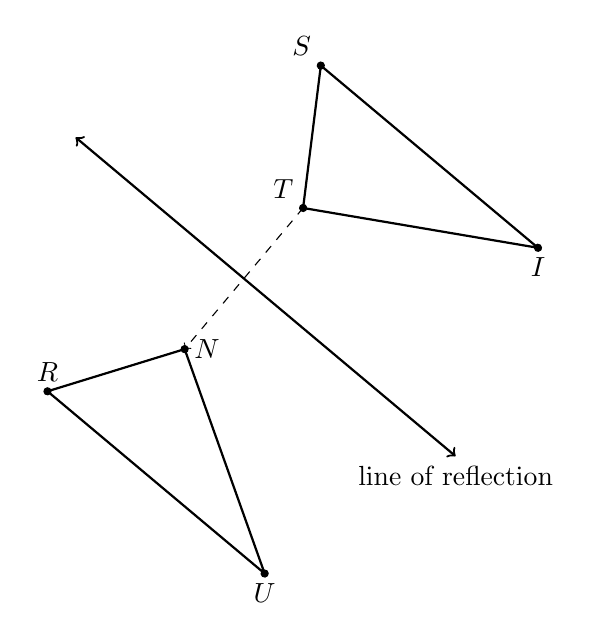
\begin{tikzpicture}[scale=0.9, rotate=-40]
      \draw [thick, <->] (0,0) -- (7,0) node [below] {line of reflection};
      \draw [dashed, ->] (3.1,1.3)--(3.1,-1.3);
      \draw [thick] (2,3)--(6,3)--(3.1,1.3)--cycle;
      \draw [thick] (2,-3)--(6,-3)--(3.1,-1.3)--cycle;
        \draw [fill] (2,3) circle [radius=0.05] node[above left] {$S$};
        \draw [fill] (2,-3) circle [radius=0.05] node[above] {$R$};
        \draw [fill] (6,3) circle [radius=0.05] node[below] {$I$};
        \draw [fill] (6,-3) circle [radius=0.05] node[below] {$U$};
        \draw [fill] (3.1,1.3) circle [radius=0.05] node[above left] {$T$};
        \draw [fill] (3.1,-1.3) circle [radius=0.05] node[right] {$N$};
    \end{tikzpicture}

    \begin{enumerate}
      \item $S \rightarrow$ \vspace{1.5cm}
      \item $T \rightarrow$ \vspace{1.5cm}
      \item $SI \rightarrow$ \vspace{1.5cm}
    \end{enumerate}
  \end{multicols}

\newpage
\item A translation maps $A$ to $A'$, as shown, $A(1,3) \rightarrow A'(4,-2)$.
\begin{multicols}{2}
  \begin{enumerate}
    \item Apply the same translation to $B(4,4)\rightarrow B'(x,y)$ on the grid. Mark and label point $B'$ as an ordered pair.
    \item Which translation mapped $A \rightarrow A'$?
    \begin{enumerate}[label=(\Alph*)]
      \item Right 3, up 1
      \item Left 3, down 1
      \item Right 5, down 3
      \item Right 3, down 5
      \item None of the above
    \end{enumerate} \vspace{2cm}

    \end{enumerate}
    \begin{flushright}
    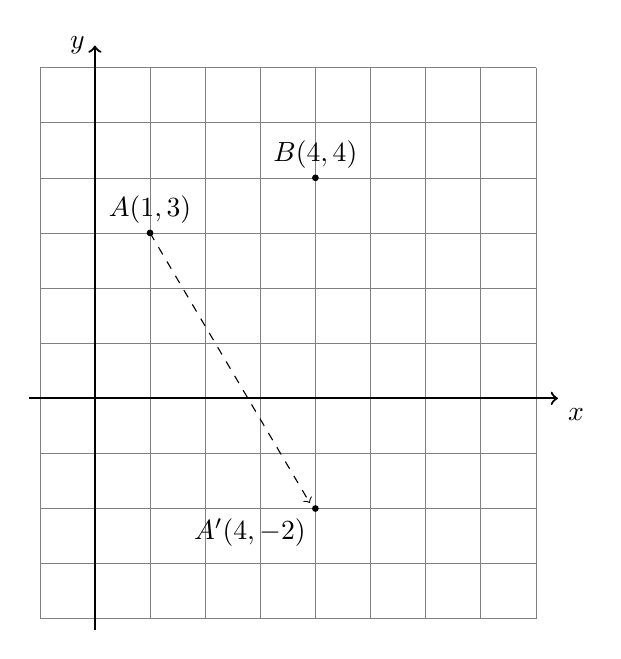
\begin{tikzpicture}[scale=0.7]
      \draw [help lines] (-1,-4) grid (8,6);
      \draw [thick, ->] (-1.2,0) -- (8.4,0) node [below right] {$x$};
      \draw [thick, ->] (0,-4.2)--(0,6.4) node [left] {$y$};
      \draw [fill] (1,3) circle [radius=0.05] node[above] {$A(1,3)$};
      \draw [fill] (4, -2) circle [radius=0.05] node[below left] {$A'(4,-2)$};
      \draw [->, dashed] (1,3)--(3.9,-1.9);
      \draw [fill] (4,4) circle [radius=0.05] node[above] {$B(4,4)$};
    \end{tikzpicture}
    \end{flushright}
\end{multicols}

\newpage
\item A $70^\circ$ clockwise rotation centered at $P$ maps $\triangle ABC \rightarrow \triangle A'B'C'$, below.
\begin{enumerate}
  \item Complete the diagram by labeling the vertices of the triangle image.\\(remember the primes)
  \item True or false: rotation is a rigid motion.
  \item Is the \emph{orientation} maintained or reversed by the rotation?
\end{enumerate}
\begin{flushright}
  \begin{tikzpicture}[scale=1.4, rotate=-10]
    \coordinate [label=above right:$A$](A) at (55:1);
    \coordinate [label=below right:$B$](B) at (2, 0);
    \coordinate [label=right:$C$](C) at (15:3.5);
    \draw [thick] (A)--(B)--(C)--cycle;
    \draw [thick, rotate=-70] (55:1) node[right]{}--
    (2,0) node[below left]{}--
    (15:3.5) node[right]{}--cycle;
    \draw [fill] (0,0) circle [radius=0.05] node[left] {$P$};
    \draw [dashed] (0,0) circle [radius=1];
  \end{tikzpicture}
\end{flushright}

\newpage
\item A reflection is performed on a line segment, mapping $\overline{AB} \rightarrow \overline{A'B'}$, as shown.
\begin{multicols}{2}
  \begin{enumerate}
    \item Apply the same reflection to $C$. \\
    Plot and label the image $C'$ as an ordered pair.
    \item Which correctly identifies the reflection?
    \begin{enumerate}[label=(\Alph*)]
      \item Reflect over the $x$-axis
      \item Reflect over the $y$-axis
      \item Reflect over the $x$-axis, then the $y$-axis
      \item Reflect over the $y$-axis, then the $x$-axis
      \item None of the above
    \end{enumerate} \vspace{2cm}
    \end{enumerate}
    \begin{flushright}
    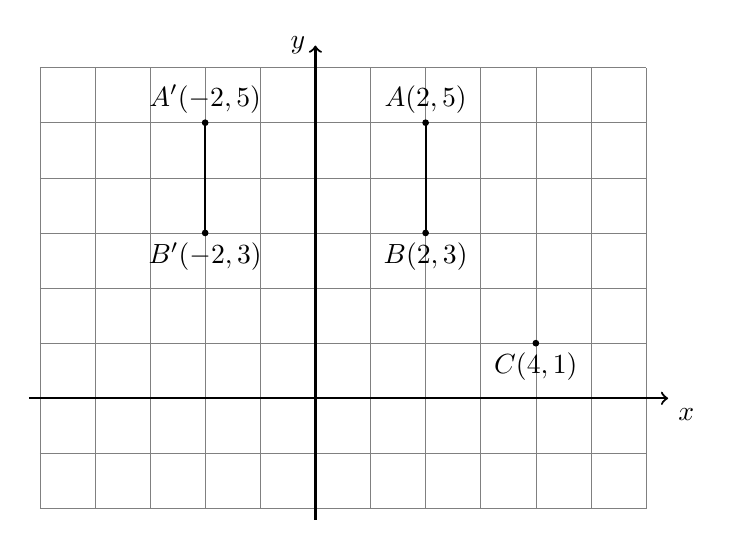
\begin{tikzpicture}[scale=0.7]
      \draw [help lines] (-5,-2) grid (6,6);
      \draw [thick, ->] (-5.2,0) -- (6.4,0) node [below right] {$x$};
      \draw [thick, ->] (0,-2.2)--(0,6.4) node [left] {$y$};
      \draw [thick] (2,5)--(2,3);
      \draw [fill] (2,5) circle [radius=0.05] node[above] {$A(2,5)$};
      \draw [fill] (2,3) circle [radius=0.05] node[below] {$B(2,3)$};
      \draw [thick] (-2,5)--(-2,3);
      \draw [fill] (-2,5) circle [radius=0.05] node[above] {$A'(-2,5)$};
      \draw [fill] (-2,3) circle [radius=0.05] node[below] {$B'(-2,3)$};
      %\draw [->, dashed] (7,1)--(2,3);
      \draw [fill] (4,1) circle [radius=0.05] node[below] {$C(4,1)$};
    \end{tikzpicture}
    \end{flushright}
\end{multicols}


\newpage
\item The transformations we study have specific details that \emph{fully characterize} the transformation. Next to each item, write the name of the appropriate transformation: translation, dilation, rotation, or reflection.
\begin{enumerate}[itemsep=0.5cm]
  \item The center and the scale factor $k$
  \item The line over which it is performed
  \item The center, the degree measure and direction
  \item The horizontal and vertical distances
\end{enumerate}

\newpage
\item What are the two transformations applied mapping $\triangle ABC \rightarrow \triangle A'B'C' \rightarrow \triangle A''B''C''$, as shown in the diagram? \emph{Fully characterize} the two transformations, in order.
    \begin{flushright}
      \includegraphics[width=6in]{5-11_6_Translate+reflect.png}
    \end{flushright}

\newpage
\item Dilate the triangle by a scale factor $k=2$ centered at the origin, $\triangle ABC \rightarrow \triangle A'B'C'$. Complete the table of the coordinates and plot and label the image on the grid. \vspace{0.5cm}
\begin{multicols}{2}
  $A(0,0) \rightarrow$ \\[0.7cm]
  $B(2,-2) \rightarrow$ \\[0.7cm]
  $C(2,0) \rightarrow$ \\[0.7cm]
    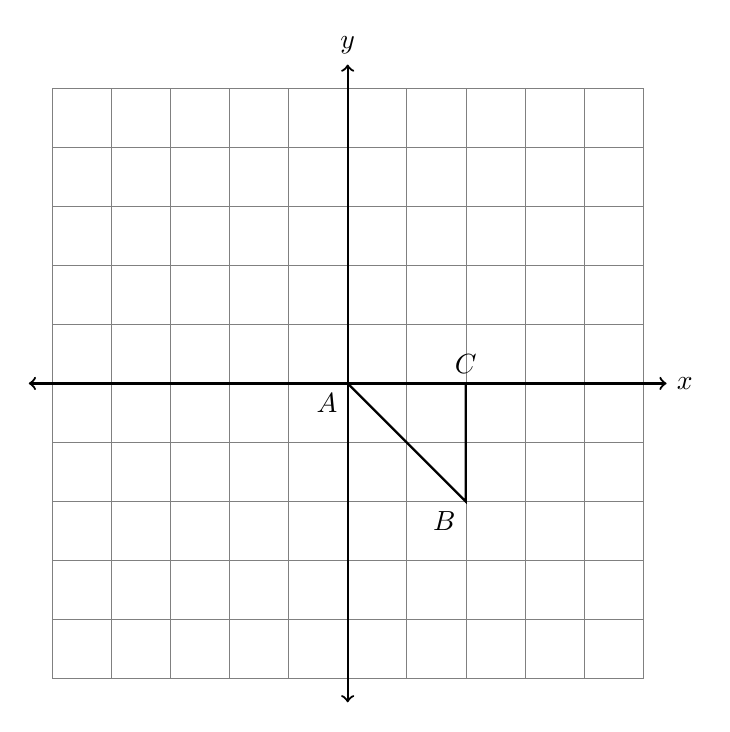
\begin{tikzpicture}[scale=.75]
    \draw [help lines] (-5,-5) grid (5,5);
    \draw [thick, <->] (-5.4,0) -- (5.4,0) node [right] {$x$};
    \draw [thick, <->] (0,-5.4)--(0,5.4) node [above] {$y$};  
    \draw [thick]
      (0,0) node[below left] {$A$}--
      (2,-2) node[below left] {$B$}--
      (2,0) node[above] {$C$}--cycle;  
    \end{tikzpicture}
  \end{multicols}

\newpage
\item Rotate the triangle $180^\circ$ counterclockwise around the origin, $\triangle ABC \rightarrow \triangle A'B'C'$. Complete the table of the coordinates and plot and label the image on the grid. \vspace{0.5cm}
\begin{multicols}{2}
  $A(0,0) \rightarrow$ \\[0.7cm]
  $B(4,2) \rightarrow$ \\[0.7cm]
  $C(4,0) \rightarrow$ \\[0.7cm]
    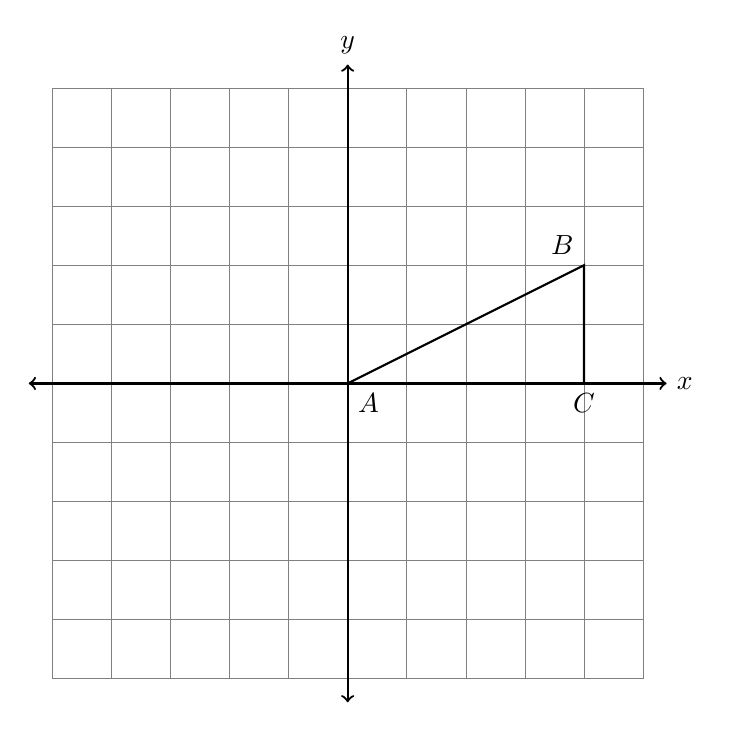
\begin{tikzpicture}[scale=.75]
    \draw [help lines] (-5,-5) grid (5,5);
    \draw [thick, <->] (-5.4,0) -- (5.4,0) node [right] {$x$};
    \draw [thick, <->] (0,-5.4)--(0,5.4) node [above] {$y$};  
    \draw [thick]
      (0,0) node[below right] {$A$}--
      (4,2) node[above left] {$B$}--
      (4,0) node[below] {$C$}--cycle;  
    \end{tikzpicture}
  \end{multicols}
  
\newpage
\item $\triangle ABC$ is shown with vertices $A(1,2)$, $B(5,1)$, and $C(6,4)$. First, translate the triangle left 7 and up 2, then reflect it across the $x$-axis. \\[0.5cm]
Plot and label $\triangle A'B'C'$ and $\triangle A''B''C''$ on the graph.
  \begin{center}
    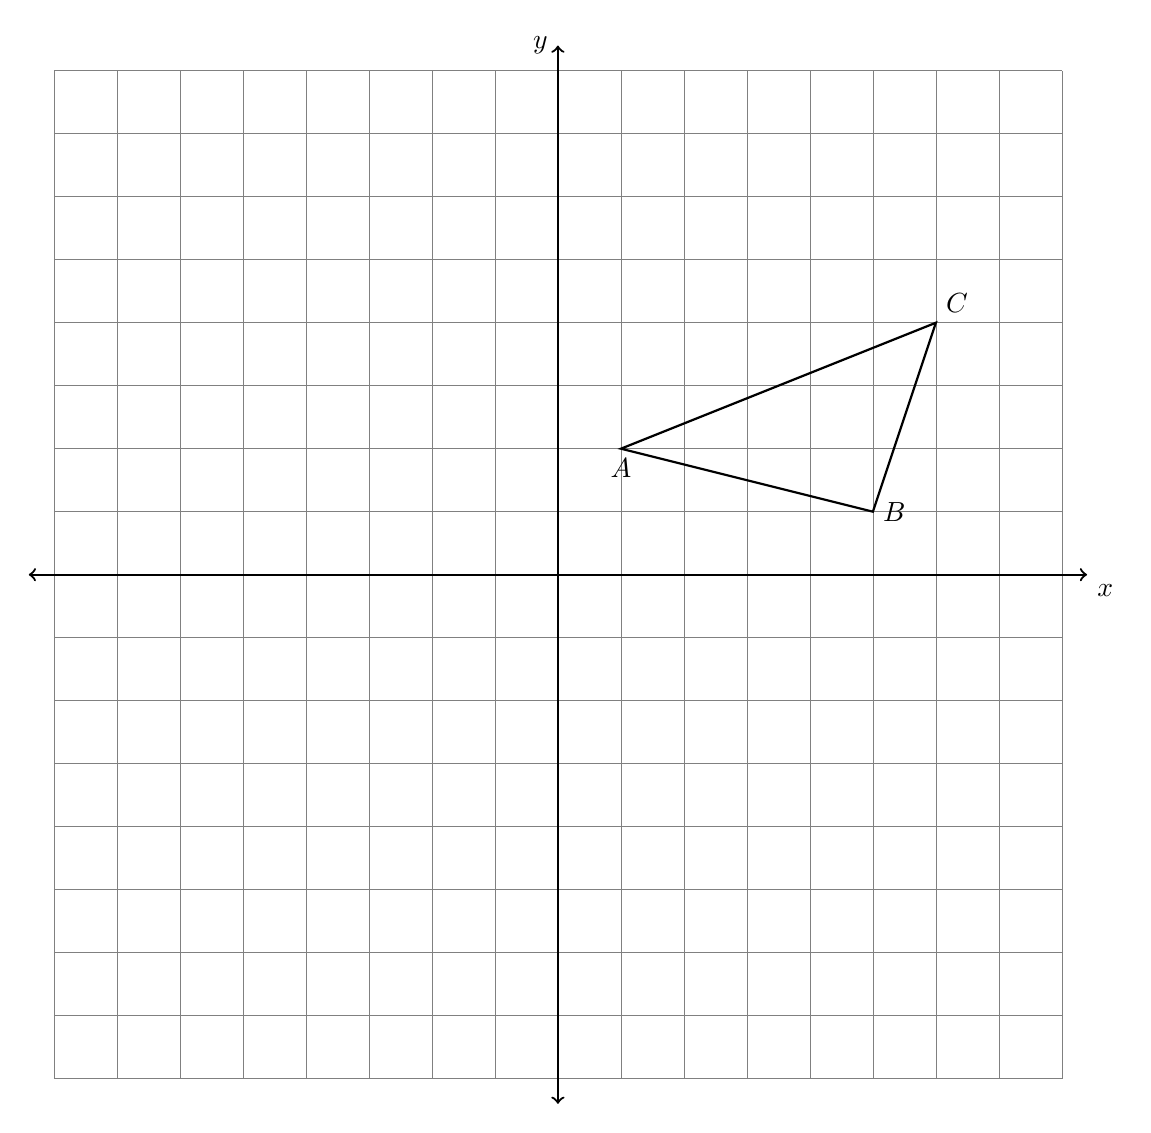
\begin{tikzpicture}[scale=0.8]
      \draw [help lines] (-8,-8) grid (8,8);
      \draw [thick, <->] (-8.4,0) -- (8.4,0) node [below right] {$x$};
      \draw [thick, <->] (0,-8.4)--(0,8.4) node [left] {$y$};
      \draw [thick] (1,2) node[below] {$A$}--
        (5,1) node[right] {$B$}--
        (6,4) node[above right] {$C$}--
        cycle;
    \end{tikzpicture}
    \end{center}

\newpage
\item A dilation centered at $A$ maps $\triangle ABC \rightarrow \triangle ADE$. Given that $BC = 10$, $DE = 15$.
  \begin{enumerate}[itemsep=1.5cm]
    \item Find the value of the scale factor $k$.
    \item Given $AB=12$, find $AD$
    \item Given $AE=12$, find $AC$
  \end{enumerate}
    \begin{flushright}
      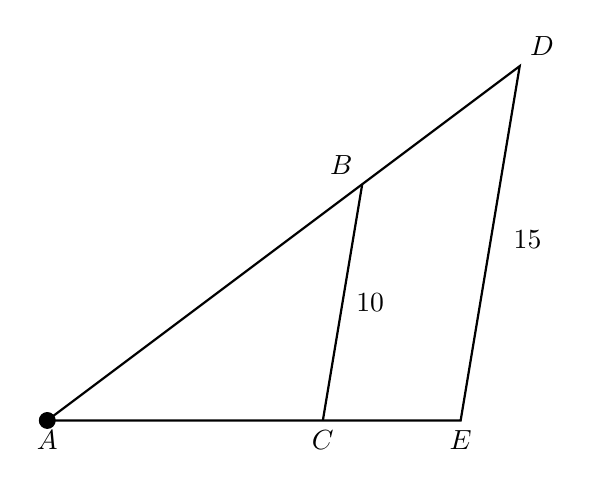
\begin{tikzpicture}[scale=1]
        \draw [-, thick] (0,0)--
        (5.25,0) node[below]{$E$}--
        (6,4.5) node[above right]{$D$}--cycle;
        \draw [thick] (3.5,0)--(4,3);
        \draw [fill] (0,0) circle [radius=0.1] node[below] {$A$};
        \node at (3.5,0) [below]{$C$};
        \node at (4,3) [above left]{$B$};
        %\node at (2, 0) [below]{$10$};
        %\node at (2, 2) [above]{$12$};
        \node at (5.8, 2.3) [right]{$15$};
        \node at (3.8, 1.5) [right]{$10$};
      \end{tikzpicture}
    \end{flushright}

\newpage
\item A point labeled $C$ and vector $(1,3)$ are shown Geogebra/classic. Identify the following objects and tools.
  \begin{enumerate}
    \item Circle the vector
    \item Make an ``X'' where to click for the menu ``Name \& Value'' that will label point $C$ as an ordered pair.
    \item Mark with an arrow the menu where the ``Translate by vector'' tool is found.
  \end{enumerate}
  \begin{flushright}
    \includegraphics[width=6in]{5-11Geogebra_toolbar.png}
  \end{flushright}

\newpage
\item Perform a composition of two transformations using Geogebra/classic. Paste an image of your work in this Classkick slide using the ``camera'' tool.
  \begin{enumerate}
    \item Plot $\triangle ABC$, $A(2,1)$, $B(5,4)$, $C(5,1)$
    \item Mark a point at the origin.
    \item Rotate the triangle $180^\circ$ counter clockwise around the origin.
    \item Reflect the image $\triangle A'B'C'$ across the $y$-axis, producing $\triangle A''B''C''$.
  \end{enumerate}
    
\end{enumerate}
\end{document}